% Options for packages loaded elsewhere
% Options for packages loaded elsewhere
\PassOptionsToPackage{unicode}{hyperref}
\PassOptionsToPackage{hyphens}{url}
\PassOptionsToPackage{dvipsnames,svgnames,x11names}{xcolor}
%
\documentclass[
  letterpaper,
  DIV=11,
  numbers=noendperiod]{scrartcl}
\usepackage{xcolor}
\usepackage{amsmath,amssymb}
\setcounter{secnumdepth}{-\maxdimen} % remove section numbering
\usepackage{iftex}
\ifPDFTeX
  \usepackage[T1]{fontenc}
  \usepackage[utf8]{inputenc}
  \usepackage{textcomp} % provide euro and other symbols
\else % if luatex or xetex
  \usepackage{unicode-math} % this also loads fontspec
  \defaultfontfeatures{Scale=MatchLowercase}
  \defaultfontfeatures[\rmfamily]{Ligatures=TeX,Scale=1}
\fi
\usepackage{lmodern}
\ifPDFTeX\else
  % xetex/luatex font selection
\fi
% Use upquote if available, for straight quotes in verbatim environments
\IfFileExists{upquote.sty}{\usepackage{upquote}}{}
\IfFileExists{microtype.sty}{% use microtype if available
  \usepackage[]{microtype}
  \UseMicrotypeSet[protrusion]{basicmath} % disable protrusion for tt fonts
}{}
\makeatletter
\@ifundefined{KOMAClassName}{% if non-KOMA class
  \IfFileExists{parskip.sty}{%
    \usepackage{parskip}
  }{% else
    \setlength{\parindent}{0pt}
    \setlength{\parskip}{6pt plus 2pt minus 1pt}}
}{% if KOMA class
  \KOMAoptions{parskip=half}}
\makeatother
% Make \paragraph and \subparagraph free-standing
\makeatletter
\ifx\paragraph\undefined\else
  \let\oldparagraph\paragraph
  \renewcommand{\paragraph}{
    \@ifstar
      \xxxParagraphStar
      \xxxParagraphNoStar
  }
  \newcommand{\xxxParagraphStar}[1]{\oldparagraph*{#1}\mbox{}}
  \newcommand{\xxxParagraphNoStar}[1]{\oldparagraph{#1}\mbox{}}
\fi
\ifx\subparagraph\undefined\else
  \let\oldsubparagraph\subparagraph
  \renewcommand{\subparagraph}{
    \@ifstar
      \xxxSubParagraphStar
      \xxxSubParagraphNoStar
  }
  \newcommand{\xxxSubParagraphStar}[1]{\oldsubparagraph*{#1}\mbox{}}
  \newcommand{\xxxSubParagraphNoStar}[1]{\oldsubparagraph{#1}\mbox{}}
\fi
\makeatother


\usepackage{longtable,booktabs,array}
\usepackage{calc} % for calculating minipage widths
% Correct order of tables after \paragraph or \subparagraph
\usepackage{etoolbox}
\makeatletter
\patchcmd\longtable{\par}{\if@noskipsec\mbox{}\fi\par}{}{}
\makeatother
% Allow footnotes in longtable head/foot
\IfFileExists{footnotehyper.sty}{\usepackage{footnotehyper}}{\usepackage{footnote}}
\makesavenoteenv{longtable}
\usepackage{graphicx}
\makeatletter
\newsavebox\pandoc@box
\newcommand*\pandocbounded[1]{% scales image to fit in text height/width
  \sbox\pandoc@box{#1}%
  \Gscale@div\@tempa{\textheight}{\dimexpr\ht\pandoc@box+\dp\pandoc@box\relax}%
  \Gscale@div\@tempb{\linewidth}{\wd\pandoc@box}%
  \ifdim\@tempb\p@<\@tempa\p@\let\@tempa\@tempb\fi% select the smaller of both
  \ifdim\@tempa\p@<\p@\scalebox{\@tempa}{\usebox\pandoc@box}%
  \else\usebox{\pandoc@box}%
  \fi%
}
% Set default figure placement to htbp
\def\fps@figure{htbp}
\makeatother





\setlength{\emergencystretch}{3em} % prevent overfull lines

\providecommand{\tightlist}{%
  \setlength{\itemsep}{0pt}\setlength{\parskip}{0pt}}



 


\usepackage{booktabs}
\usepackage{longtable}
\usepackage{array}
\usepackage{multirow}
\usepackage{wrapfig}
\usepackage{float}
\usepackage{colortbl}
\usepackage{pdflscape}
\usepackage{tabu}
\usepackage{threeparttable}
\usepackage{threeparttablex}
\usepackage[normalem]{ulem}
\usepackage{makecell}
\usepackage{xcolor}
\usepackage{caption}
\usepackage{anyfontsize}
\KOMAoption{captions}{tableheading}
\makeatletter
\@ifpackageloaded{caption}{}{\usepackage{caption}}
\AtBeginDocument{%
\ifdefined\contentsname
  \renewcommand*\contentsname{Table of contents}
\else
  \newcommand\contentsname{Table of contents}
\fi
\ifdefined\listfigurename
  \renewcommand*\listfigurename{List of Figures}
\else
  \newcommand\listfigurename{List of Figures}
\fi
\ifdefined\listtablename
  \renewcommand*\listtablename{List of Tables}
\else
  \newcommand\listtablename{List of Tables}
\fi
\ifdefined\figurename
  \renewcommand*\figurename{Figure}
\else
  \newcommand\figurename{Figure}
\fi
\ifdefined\tablename
  \renewcommand*\tablename{Table}
\else
  \newcommand\tablename{Table}
\fi
}
\@ifpackageloaded{float}{}{\usepackage{float}}
\floatstyle{ruled}
\@ifundefined{c@chapter}{\newfloat{codelisting}{h}{lop}}{\newfloat{codelisting}{h}{lop}[chapter]}
\floatname{codelisting}{Listing}
\newcommand*\listoflistings{\listof{codelisting}{List of Listings}}
\makeatother
\makeatletter
\makeatother
\makeatletter
\@ifpackageloaded{caption}{}{\usepackage{caption}}
\@ifpackageloaded{subcaption}{}{\usepackage{subcaption}}
\makeatother
\usepackage{bookmark}
\IfFileExists{xurl.sty}{\usepackage{xurl}}{} % add URL line breaks if available
\urlstyle{same}
\hypersetup{
  pdftitle={Energy Audit Report},
  colorlinks=true,
  linkcolor={blue},
  filecolor={Maroon},
  citecolor={Blue},
  urlcolor={Blue},
  pdfcreator={LaTeX via pandoc}}


\title{Energy Audit Report}
\author{}
\date{}
\begin{document}
\maketitle


\textbf{Homeowner(s):} Jackie Lola

\textbf{Address:} 106 Thunder Road Perry, Maine, 04667

\textbf{Owner Contact:} NA

\textbf{Auditors:} Helen Lloyd, Tyler Hebert, Raquel Longfellow

\textbf{Contact:} David Gibson, dgibson@coa.edu, (802) 266-0301

\textbf{Report Date:} July 11, 2025

\begin{center}\rule{0.5\linewidth}{0.5pt}\end{center}

We conducted an energy assessment of your home on 7/10/2025. This report
will tell you what we did, what we found, and what we suggest for your
home. These suggestions include information on incentives and financing
to make improvements more affordable.

\begin{center}\rule{0.5\linewidth}{0.5pt}\end{center}

\begin{center}
\pandocbounded{\includegraphics[keepaspectratio]{images/Logos-together.png}}
\end{center}

\newpage{}

\textbf{Add here the table of content: in Word go to references and add
table of content, in Docs go to the insert and on the bottom add the
table of context}

\newpage{}

\subsection{Summary of your Audit}\label{summary-of-your-audit}

\subsubsection{Visual Inspection and
Measurements}\label{visual-inspection-and-measurements}

We started with a tour and visual inspection of the inside and outside
of the home. We identified any visible damage to the building, moisture
control strategies, major appliances, and insulation. We measured square
footage and volume of the home, as well as the area of all exterior
windows and doors. We used a kill-a-watt meter to measure the
electricity use of some appliances. During your audit, we used a carbon
monoxide meter to measure the ambient carbon monoxide levels throughout
the home.

\subsubsection{Attic}\label{attic}

We entered the attic to check for insulation, air sealing, ventilation,
and potential hazards such as mold. Additionally, we visually inspected
the attic ventilation and any duct and pipework passing through the
attic.

\subsubsection{Basement}\label{basement}

We visually inspected any appliances in the basement and noted
insulation levels, moisture, rodents, and any other concerns.

\subsubsection{Blower Door / Air Leakage
Test}\label{blower-door-air-leakage-test}

A blower door test measures the air tightness of a building. We used a
specialized fan in an exterior door to generate negative pressure inside
your house. The resulting pressure difference between the inside and
outside of the house allows us to measure air leakage. To locate the
leaks, we used an infrared camera to check for unusually hot and cold
spots. We also checked the pressure differences of the rooms to help
determine major air leak locations.

\subsubsection{Combustion Appliance
Safety}\label{combustion-appliance-safety}

We assessed combustion appliances that burn fossil fuels such as
propane, heating oil, or kerosene. These include furnaces, boilers,
water heaters, and gas ovens. We visually inspected the combustion
appliance(s) in your home, but we were unable to perform combustion
safety tests. We also performed gas leak detection tests on your propane
appliance(s).

\newpage{}

\subsection{Summary of
Recommendations}\label{summary-of-recommendations}

We recommend the following upgrades for your home. Detailed information
about these recommendations and financial resources can be found in
other sections of this report. These are organized from the least
expensive/most cost-effective and easiest interventions to ones that are
more challenging to implement.

\begin{table}
\fontsize{12.0pt}{14.4pt}\selectfont
\begin{tabular*}{1\linewidth}{@{\extracolsep{\fill}}>{\raggedright\arraybackslash}p{\dimexpr 150.00pt -2\tabcolsep-1.5\arrayrulewidth}>{\raggedright\arraybackslash}p{\dimexpr 337.50pt -2\tabcolsep-1.5\arrayrulewidth}}
\toprule
Recommendations & Description \\ 
\midrule\addlinespace[2.5pt]
Solar & Rooftop solar can supply most or all of your home electrical demands. Contact a solar company for pricing and details specific to your home. \\ 
Misc. Air Sealing and Insulation & Air seal and insulate [** insert auditor description - bay window, bulkhead door, chase, kneewall, anything else that is unique to the home and not otherwise covered in another recommendation] \\ 
Furnace/Boiler Tune-up & Have the furnace/boiler and flue inspected and adjusted by a licensed professional. This should be available from your fuel delivery company. \\ 
High-efficiency Shower Head(s) & Install high-efficiency shower heads to reduce the amount of water and energy to heat the water used when showering. \\ 
LEDs & Switch your light bulbs to LED light bulbs. LEDs use 80\% less energy than incandescent light bulbs, which can significantly reduce your electricity bill. \\ 
Refrigerator & Replace your refrigerator with a new, EnergyStar-certified fridge. Look at the Energy Guide label to compare the energy use of new refrigerators. \\ 
Induction Stove/Oven & Induction cooking appliances are more efficient and safer than electric or gas ones. There is no risk of carbon monoxide or other harmful combustion gases, and the surface doesn’t heat up without a pot or pan on it. \\ 
Gutters & Install gutters and downspouts that divert water at least six feet away from the foundation and to where the ground slopes away from the house. \\ 
Bathroom Exhaust Fan(s) & Install bathroom exhaust fans in all bathrooms that do not have them. These should be rated for at least 80 cubic feet per minute (CFM) if there is a shower. We recommend the Panasonic Whisper series or similar fans that don’t create excess noise. \\ 
Kitchen Exhaust Fan & Install a kitchen exhaust fan to remove cooking fumes and moisture from your home. The fan should be rated for at least 100 cubic feet per minute. A kitchen fan should be ducted to the outdoors. If the ductwork will run through the attic, it should be installed before the attic is air-sealed and insulated. \\ 
Vapor Barrier & Install a vapor barrier on the basement floor to stop moisture from entering the basement and house. \\ 
Spray Foam Basement/Crawlspace Walls & Install spray foam on the basement/crawlspace walls to prevent moisture infiltration and reduce heat loss. \\ 
Attic Air Sealing and Insulation & Air seal the attic and insulate it to at least R-60 (18 inches of loose-fill cellulose insulation). \\ 
Continuous Exterior Wall Insulation & Add a continuous layer of insulation and potentially replace the air and moisture barrier once it becomes time to replace the siding. \\ 
Electrical Panel Upgrade & Consult with an electrician about replacing your existing electrical panel with a 200 amp panel as you add electrical appliances to your home. \\ 
Air Source Heat Pump & Install air source heat pumps for heating and cooling and whole-house surge protection. \\ 
Whole-House Surge Protection & Upgrade your electrical panel to add whole-house surge protection. \\ 
Pipe Insulation & Insulate both hot and cold water pipes that are uninsulated in the basement/crawlspace. This will save energy and prevent condensation. \\ 
Other 1 & TYPE HERE 1 \\ 
Heat Pump Water Heater & Install a heat pump water heater to provide your hot water for cooking and bathing. This is the most efficient way to heat water and will save hundreds of dollars a year compared to electric resistance, heating oil, or propane hot water. It will also help to dehumidify while it's running. If your current water heater burns oil or propane, this will also remove a source of combustion gases from your home. \\ 
\bottomrule
\end{tabular*}
\end{table}

\newpage{}

\subsection{What We Found}\label{what-we-found}

\subsubsection{Basics}\label{basics}

\begin{table}
\fontsize{9.0pt}{10.8pt}\selectfont
\begin{tabular*}{1\linewidth}{@{\extracolsep{\fill}}>{\centering\arraybackslash}p{\dimexpr 150.00pt -2\tabcolsep-1.5\arrayrulewidth}>{\raggedright\arraybackslash}p{\dimexpr 337.50pt -2\tabcolsep-1.5\arrayrulewidth}}
\toprule
Info & Values \\ 
\midrule\addlinespace[2.5pt]
Date Built: & 1992 \\ 
Foundation Type: & Crawlspace \\ 
Attic: & Batts of Fiberglass , 9 inches \\ 
Number of floors: & 2 \\ 
Square footage of conditioned space: & 1,535 ft² \\ 
Volume of conditioned space: & 11,863 ft³ \\ 
Ambient Carbon Monoxide reading: & 0 \\ 
\bottomrule
\end{tabular*}
\end{table}

\subsubsection{Exterior}\label{exterior}

\begin{table}
\fontsize{12.0pt}{14.4pt}\selectfont
\begin{tabular*}{1\linewidth}{@{\extracolsep{\fill}}>{\raggedright\arraybackslash}p{\dimexpr 150.00pt -2\tabcolsep-1.5\arrayrulewidth}>{\raggedright\arraybackslash}p{\dimexpr 337.50pt -2\tabcolsep-1.5\arrayrulewidth}}
\toprule
Info & Values \\ 
\midrule\addlinespace[2.5pt]
Roof age: & 15 \\ 
Orientation: & Northeast/Southwest \\ 
Roof type: & The house has a Asphalt Shingles roof.The roof is in NA condition. The shingles show clear signs of age and weathering. They have not begun to fly away during wind events. \\ 
Moisture control: & The house has the following moisture control strategies: NA.  These were in NA condition. NA \\ 
Siding: & The house has vinyl siding. The siding is in fair condition. The siding is in good condition in most areas. There are some spots that have had cracks or breaks in the material. \\ 
Exterior doors: & There are 2 hollow fiberglass exterior doors. These are in excellent condition, they have a total area of 37 ft². \\ 
Exterior windows: & There are 13 double paned wood windows. These are in fair condition, they have a total area of 148 ft². \\ 
\bottomrule
\end{tabular*}
\end{table}

\subsubsection{Interior/Living space}\label{interiorliving-space}

\begin{table}
\fontsize{12.0pt}{14.4pt}\selectfont
\begin{tabular*}{1\linewidth}{@{\extracolsep{\fill}}>{\raggedright\arraybackslash}p{\dimexpr 112.50pt -2\tabcolsep-1.5\arrayrulewidth}>{\raggedright\arraybackslash}p{\dimexpr 75.00pt -2\tabcolsep-1.5\arrayrulewidth}}
\toprule
Info & Values \\ 
\midrule\addlinespace[2.5pt]
Walls: & The house has platform framing, which means that wall cavities do not extend the full height of the building, but are instead separated by floors. The exterior walls are insulated with Batts of Fiberglass insulation. This insulation is 4 inches thick and in fair condition. This gives the exterior walls an R-value of around CALCULATE. A material’s R-value tells us how good it is at stopping heat flow, the bigger the number, the better. For comparison, current Maine building code requires an R-value of at least R-13 with additional continuous insulation of R-10 for exterior walls or R-20 with additional continuous insulation of R-5. The insulation in the walls was installed during the construction of the home. \\ 
Living room: & NA \\ 
Bathroom(s): & NA \\ 
Kitchen: & During the audit we measured the electricity consumption of the Fridge and Freezer Combo. It used NA kWh in NA hours. We thus estimate that it is costing you around \$CALCULATE a month to run. This is **comparable to / more expensive than** newer, efficient models. The Chest Freezer used NA kWh in NA hours.  We thus estimate that it is costing you around \$CALCULATE a month to run. This is **comparable to / more expensive than** newer, efficient models. The dishwasher is on the older side and is too loud for the homeowner's liking. \\ 
\bottomrule
\end{tabular*}
\end{table}

\begin{table}
\fontsize{8.2pt}{9.9pt}\selectfont
\begin{tabular*}{\linewidth}{@{\extracolsep{\fill}}lll}
\toprule
 &  &  \\ 
\midrule\addlinespace[2.5pt]
CFM50: & 1250 & CFM50 describes how many cubic feet per minute of air are leaving the house at 50 pascals of pressure difference (while the blower door is running). For every cubic foot of air that leaves the house, a cubic foot of air enters the house as well. The higher the number, the leakier the house. \\ 
ACH50: & 6.3 & ACH50 tells us how many air changes per hour are taking place in the house at 50 pascals of pressure difference. This value is normalized for the volume of the house and thus allows for comparison between different houses. The higher the number, the leakier the house. \\ 
Equivalent leakage area: & 125 in² under natural conditions. & This is the area (in square inches) equivalent to all of the air leaks in the house combined. \\ 
ACHnatural: & 0.5 & Accounting for the volume of the home, this means that the house exchanges –\% of its air every hour. Over one day, the house goes through – complete air changes. \\ 
\bottomrule
\end{tabular*}
\end{table}

\subsubsection{Blower Door / Air Leakage
Test}\label{blower-door-air-leakage-test-1}

\{r\} \#\textbar{} label: blower door data set up for 3.4 \#\textbar{}
echo: false

\#old set up wiht manual entry to googlespreadsheet
blower\_door\_leakage \textless-
energy\_test\_googlesheets\textbar\textgreater{} select( ``Equivalent
leakage area'')\textbar\textgreater{}
mutate(\texttt{Equivalent\ leakage\ area} =
paste0(\texttt{Equivalent\ leakage\ area}, '' in²''))

\#blower\_door\_leakage \textless-blower\_door\_leakage{[},-c(1){]}

blower\_door\_leakage
\textless-blower\_door\_leakage\textbar\textgreater{}
pivot\_longer(c(``Equivalent leakage area''), names\_to = ``Info'',
values\_to = ``Values'')

blower\_door \textless- energy\_test\_googlesheets\textbar\textgreater{}
select(c(``CFM50'', ``ACH50'',``ACHn'', ))\textbar\textgreater{} \#there
is another column ``Comments about air leakage''
pivot\_longer(c(``CFM50'', ``ACH50'',``ACHn''), names\_to = ``Info'',
values\_to = ``Values'')

all\_blower\_door \textless- blower\_door\textbar\textgreater{}
rbind(blower\_door\_leakage)\textbar\textgreater{} mutate(Info =
recode(Info, ``CFM50'' = ``CFM50:'', ``ACH50'' = ``ACH50:'',``Equivalent
leakage area'' = ``Equivalent leakage area:'',``ACHn'' = ``ACHnatural:''
))\textbar\textgreater{} arrange(factor(Info, levels = c(`CFM50:',
`ACH50:', `Equivalent leakage area:', `ACHnatural:')))

all\_blower\_door{[}`Description'{]} \textless- c(``CFM50 describes how
many cubic feet per minute of air are leaving the house at 50 pascals of
pressure difference (while the blower door is running). For every cubic
foot of air that leaves the house, a cubic foot of air enters the house
as well. The higher the number, the leakier the house.'', ``ACH50 tells
us how many air changes per hour are taking place in the house at 50
pascals of pressure difference. This value is normalized for the volume
of the house and thus allows for comparison between different houses.
The higher the number, the leakier the house.'',``This is the area (in
square inches) equivalent to all of the air leaks in the house
combined.'',``Accounting for the volume of the home, this means that the
house exchanges --\% of its air every hour. Over one day, the house goes
through -- complete air changes.'')

\{r\} \#\textbar{} label: ACH/CFM/ELA/N-factor calculations \#\textbar{}
echo: false

table\_3\_4 \textless-clean\_audit\_data\textbar\textgreater{}
select(cfm50)

table\_3\_4\textless- as.data.frame(as.numeric(table\_3\_4))

\#ACH50 calculation

table\_3\_4\(ACH50_cal <- as.numeric(clean_audit_data\)cfm50) * 60 /
as.numeric(clean\_audit\_data\$volume\_of\_conditioned\_space\_cubic\_feet)

\#Equivalent leakage area calculation

table\_3\_4\(equi_leak_area_cal <- (as.numeric(clean_audit_data\)cfm50)
/ 10)

\#N-factor calculation

n\_factor\_calculated \textless- clean\_audit\_data
\textbar\textgreater{} select(exposure\_of\_the\_house,
number\_of\_floors)\textbar\textgreater{} mutate(n\_factor\_cal =
case\_when( exposure\_of\_the\_house == ``Low'' \& number\_of\_floors ==
1 \textasciitilde{} 22.2, exposure\_of\_the\_house == ``Low'' \&
number\_of\_floors == 1.5 \textasciitilde{} 20.0,
exposure\_of\_the\_house == ``Low'' \& number\_of\_floors == 2
\textasciitilde{} 17.8, exposure\_of\_the\_house == ``Low'' \&
number\_of\_floors == 3 \textasciitilde{} 15.5, exposure\_of\_the\_house
== ``Moderate'' \& number\_of\_floors == 1 \textasciitilde{} 18.5,
exposure\_of\_the\_house == ``Moderate'' \& number\_of\_floors == 1.5
\textasciitilde{} 16.7, exposure\_of\_the\_house == ``Moderate'' \&
number\_of\_floors == 2 \textasciitilde{} 14.8, exposure\_of\_the\_house
== ``Moderate'' \& number\_of\_floors == 3 \textasciitilde{} 13.0,
exposure\_of\_the\_house == ``High'' \& number\_of\_floors == 1
\textasciitilde{} 16.7, exposure\_of\_the\_house == ``High'' \&
number\_of\_floors == 1.5 \textasciitilde{} 15.0,
exposure\_of\_the\_house == ``High'' \& number\_of\_floors == 2
\textasciitilde{} 13.3, exposure\_of\_the\_house == ``High'' \&
number\_of\_floors == 3 \textasciitilde{} 11.7))

\#CFM natural calculation (Do I need to even calculate it)

\#table\_3\_4\(CFMnatural_cal <- as.numeric(n_factor_calculated\)n\_factor\_cal)/
as.numeric(clean\_audit\_data\$cfm50)

\#ACH natural calculation

table\_3\_4\(ACHnatural_cal <- as.numeric(table_3_4\)ACH50\_cal)/
as.numeric(n\_factor\_calculated\$n\_factor\_cal)

table\_3\_4 \textless- table\_3\_4\textbar\textgreater{}
mutate(across(where(\textasciitilde{} is.numeric(.)), \textasciitilde{}
round(., 1)))

\#Clean the data frame

table\_3\_4 \textless- cbind(table\_3\_4,
n\_factor\_calculated)\textbar\textgreater{}
select(-c(5,6,7))\textbar\textgreater{} pivot\_longer( cols =
everything(), names\_to = ``Info'', values\_to = ``Values'')

equi\_leak\_area \textless- table\_3\_4{[}3,{]} equi\_leak\_area
\textless- table\_3\_4{[}3,{]}\textbar\textgreater{} mutate(Values=
paste0(equi\_leak\_area\$Values, '' under natural conditions. TEST''))

table\_3\_4 \textless- table\_3\_4\textbar\textgreater{}
rbind(equi\_leak\_area)

table\_3\_4 \textless- table\_3\_4{[}-3,{]}

table\_3\_4 \textless- table\_3\_4\textbar\textgreater{} mutate(Info =
recode(Info, ``as.numeric(table\_3\_4)'' = ``CFM50:'', ``ACH50\_cal'' =
``ACH50:'',``equi\_leak\_area\_cal'' = ``Equivalent leakage
area:'',``ACHnatural\_cal'' = ``ACHnatural:'' ))\textbar\textgreater{}
arrange(factor(Info, levels = c(`CFM50:', `ACH50:', `Equivalent leakage
area:', `ACHnatural:')))

table\_3\_4{[}`Description'{]} \textless- c(``CFM50 describes how many
cubic feet per minute of air are leaving the house at 50 pascals of
pressure difference (while the blower door is running). For every cubic
foot of air that leaves the house, a cubic foot of air enters the house
as well. The higher the number, the leakier the house.'', ``ACH50 tells
us how many air changes per hour are taking place in the house at 50
pascals of pressure difference. This value is normalized for the volume
of the house and thus allows for comparison between different houses.
The higher the number, the leakier the house.'',``This is the area (in
square inches) equivalent to all of the air leaks in the house
combined.'',``Accounting for the volume of the home, this means that the
house exchanges --\% of its air every hour. Over one day, the house goes
through -- complete air changes.'')

A blower door test simulates a 20mph wind hitting your house from all
sides.

To run the test, we used a large fan in an exterior door to depressurize
your house. As air is pulled out through the fan, an equal volume of air
is pulled in through all of the gaps, cracks, and air leaks throughout
the house. This allows us to determine the volume of air leakage into
the house and to locate bigger air leaks.

To find leaks, we used an infrared camera to check for unusually hot and
cold spots. We also checked the pressure differences of the rooms to
help determine major air leak locations.

Air leaks are a big source of heat gain in warm weather and heat loss in
cold weather. They also allow moisture to get into the home. Below are
some numbers, pictures, and descriptions explaining what we found.

\begin{table}
\fontsize{12.0pt}{14.4pt}\selectfont
\begin{tabular*}{1\linewidth}{@{\extracolsep{\fill}}>{\centering\arraybackslash}p{\dimexpr 112.50pt -2\tabcolsep-1.5\arrayrulewidth}>{\raggedright\arraybackslash}p{\dimexpr 75.00pt -2\tabcolsep-1.5\arrayrulewidth}>{\raggedright\arraybackslash}p{\dimexpr 300.00pt -2\tabcolsep-1.5\arrayrulewidth}}
\toprule
Info & Values & Description \\ 
\midrule\addlinespace[2.5pt]
CFM50: & 1250 & CFM50 describes how many cubic feet per minute of air are leaving the house at 50 pascals of pressure difference (while the blower door is running). For every cubic foot of air that leaves the house, a cubic foot of air enters the house as well. The higher the number, the leakier the house. \\ 
ACH50: & 6.3 & ACH50 tells us how many air changes per hour are taking place in the house at 50 pascals of pressure difference. This value is normalized for the volume of the house and thus allows for comparison between different houses. The higher the number, the leakier the house. \\ 
Equivalent leakage area: & 125 in² under natural conditions. & This is the area (in square inches) equivalent to all of the air leaks in the house combined. \\ 
ACHnatural: & 0.5 & Accounting for the volume of the home, this means that the house exchanges –\% of its air every hour. Over one day, the house goes through – complete air changes. \\ 
\bottomrule
\end{tabular*}
\end{table}

\pandocbounded{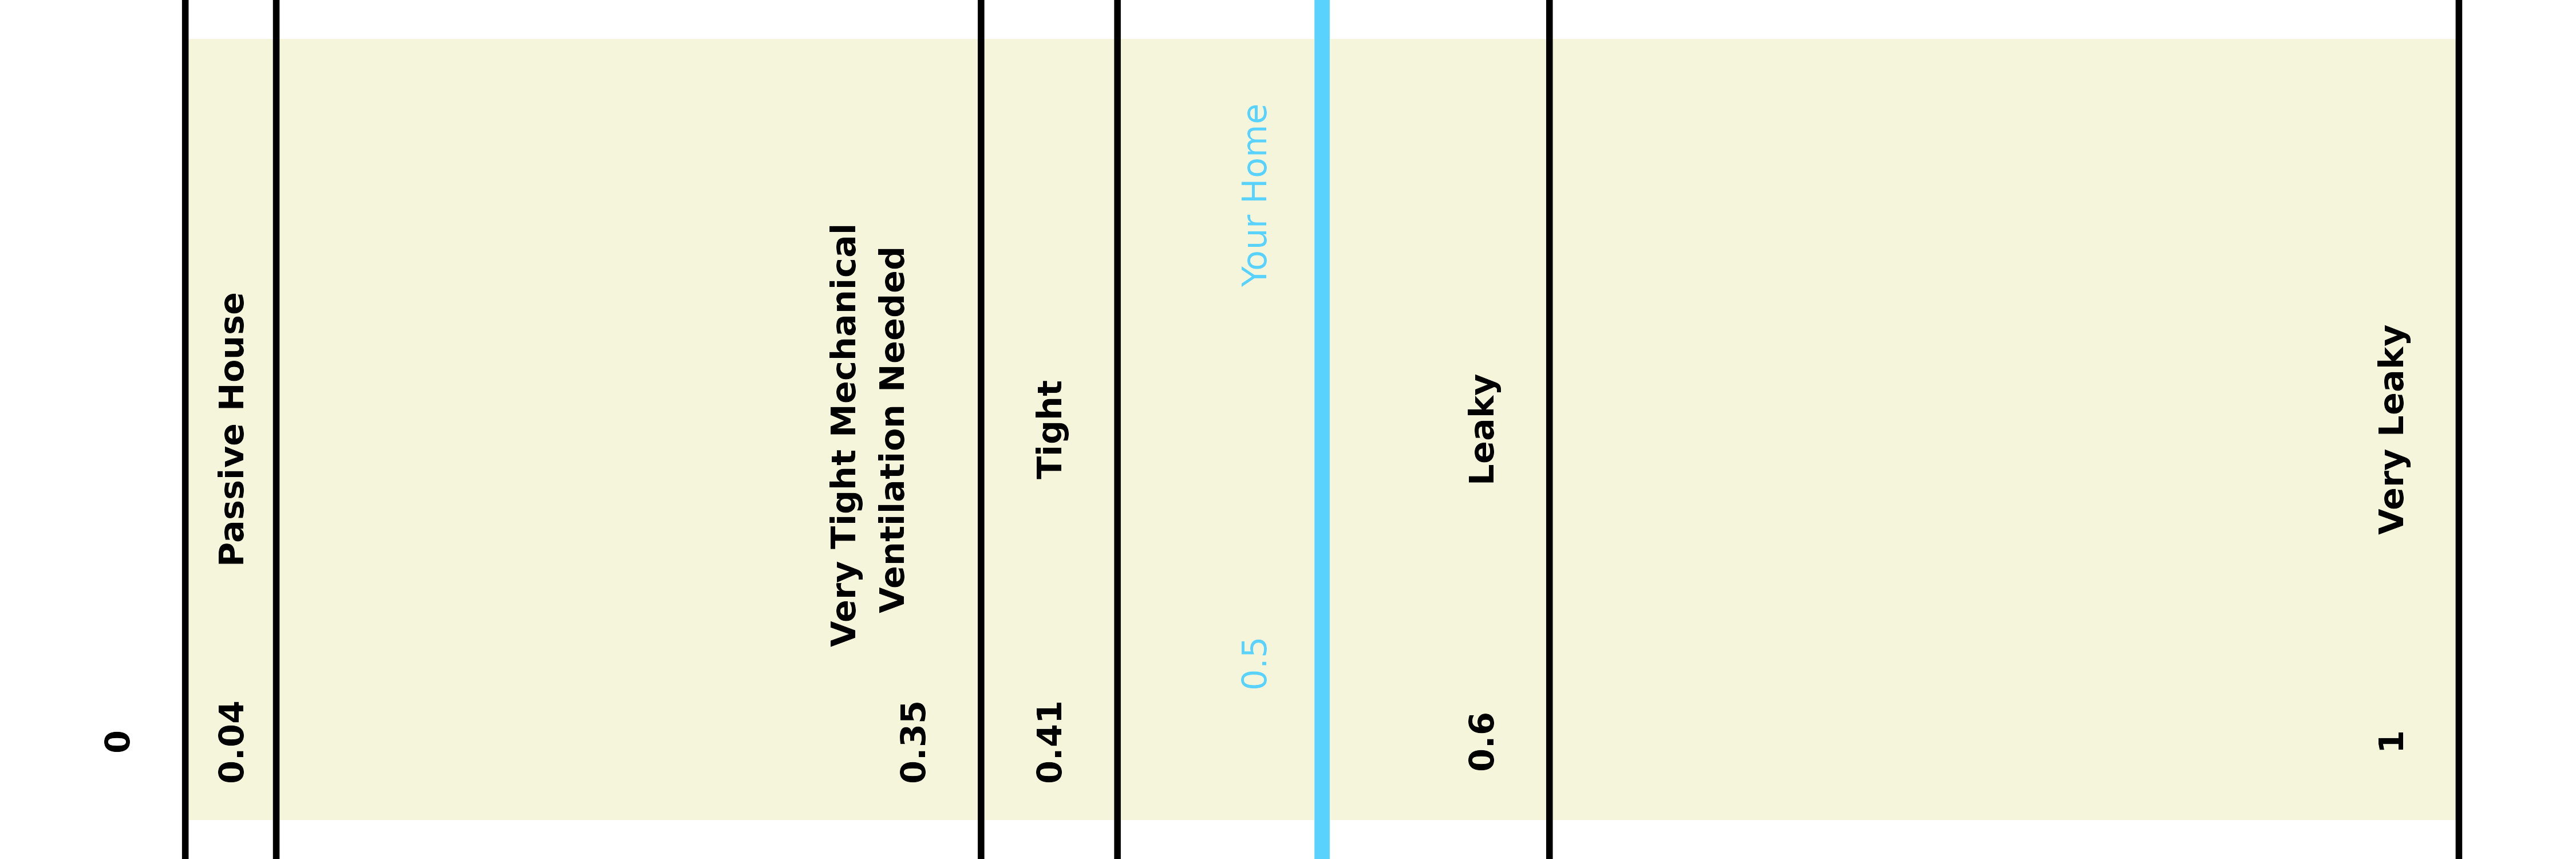
\includegraphics[keepaspectratio]{achnatural_ggplot1.png}}

\emph{Your house compared to standards}

Using a thermal imaging camera, we looked for major air leakage
locations and thermal bridging. Thermal bridging occurs when heat enters
or leaves a house through material that lets heat through more easily
than the house's insulation. This often occurs with wall studs and
ceiling joists.

We conducted the audit in the summer, when the air outside the house is
hotter than inside the house. Therefore, the warmer (red, orange, and
yellow) areas in the thermal pictures below show where air leakage is
taking place, as these are the areas where hot air from the outside is
being pulled into the cooler house.

\subsubsection{Attic}\label{attic-1}

\begin{table}
\fontsize{9.0pt}{10.8pt}\selectfont
\begin{tabular*}{1\linewidth}{@{\extracolsep{\fill}}>{\raggedright\arraybackslash}p{\dimexpr 150.00pt -2\tabcolsep-1.5\arrayrulewidth}>{\raggedright\arraybackslash}p{\dimexpr 337.50pt -2\tabcolsep-1.5\arrayrulewidth}}
\toprule
Info & Values \\ 
\midrule\addlinespace[2.5pt]
{Area:} & {586.5} \\ 
{Insulation type:} & {Batts of Fiberglass} \\ 
{Insulation condition:} & {Fair} \\ 
{Air sealing:} & {There is Noair sealing. NA} \\ 
{Other observations:} & {The attic is mostly insulated, some spots have poorly installed fiberglass batts or lack insulation completely. Rodents have begun eating away at the insulation. The chimney is not air sealed, and opens up into an open cavity that is uninsulated. No NA} \\ 
{Ventilation:} & {No} \\ 
{Ducts:} & {No} \\ 
\bottomrule
\end{tabular*}
\end{table}

\subsubsection{Basement}\label{basement-1}

\begin{table}
\fontsize{12.0pt}{14.4pt}\selectfont
\begin{tabular*}{1\linewidth}{@{\extracolsep{\fill}}>{\raggedright\arraybackslash}p{\dimexpr 150.00pt -2\tabcolsep-1.5\arrayrulewidth}>{\raggedright\arraybackslash}p{\dimexpr 337.50pt -2\tabcolsep-1.5\arrayrulewidth}}
\toprule
Info & Values \\ 
\midrule\addlinespace[2.5pt]
Area: & 890 \\ 
Insulation condition: & FairThe crawlspace has 2" foam board insulation on the interior walls, as well as 4" fiberglass batts in the rim joists. \\ 
Insulation type: & Batts of Fiberglass, Rigid foam board \\ 
Insulation of appliances: & Appliances not insulated, Ducts/pipes not insulated \\ 
Moisture Control: & NAin NAcondition. NA \\ 
Ducts: & NoNA \\ 
Other observations: & There is NANA \\ 
\bottomrule
\end{tabular*}
\end{table}

\subsubsection{Electrical and Mechanical
Systems}\label{electrical-and-mechanical-systems}

\begin{table}
\fontsize{12.0pt}{14.4pt}\selectfont
\begin{tabular*}{1\linewidth}{@{\extracolsep{\fill}}>{\raggedright\arraybackslash}p{\dimexpr 150.00pt -2\tabcolsep-1.5\arrayrulewidth}>{\raggedright\arraybackslash}p{\dimexpr 337.50pt -2\tabcolsep-1.5\arrayrulewidth}}
\toprule
Info & Values \\ 
\midrule\addlinespace[2.5pt]
Electrical panel: & The electrical panel has and  amperage of 100. There are 0 unused breaker spaces. The homeowner has a full panel and is in fine condition. \\ 
\bottomrule
\end{tabular*}
\end{table}

\subsubsection{Energy Bills}\label{energy-bills}

\begin{table}
\fontsize{12.0pt}{14.4pt}\selectfont
\begin{tabular*}{1\linewidth}{@{\extracolsep{\fill}}>{\raggedright\arraybackslash}p{\dimexpr 165.00pt -2\tabcolsep-1.5\arrayrulewidth}>{\raggedleft\arraybackslash}p{\dimexpr 165.00pt -2\tabcolsep-1.5\arrayrulewidth}l>{\raggedleft\arraybackslash}p{\dimexpr 165.00pt -2\tabcolsep-1.5\arrayrulewidth}}
\toprule
Type & kWh/gallons/cords/tonns & Type2 & Cost (USD) \\ 
\midrule\addlinespace[2.5pt]
Propane & 302.3 & cost\_in\_dollars\_propane & 1035.3 \\ 
Electricity & 2700 & cost\_in\_dollars\_electricity & 259 \\ 
\bottomrule
\end{tabular*}
\end{table}

\newpage{}

\subsection{Recommendations}\label{recommendations}

These recommendations are organized from the least expensive/most
cost-effective and easiest interventions to ones that are more
challenging to implement.

\subsubsection{Furnace/Boiler Tune up}\label{furnaceboiler-tune-up}

\emph{Problem}

\textbf{Auditor to describe}

\emph{Recommendation}

Have the furnace/boiler and flue inspected and adjusted by a licensed
professional. This should be available from your fuel delivery company.

\emph{Estimated Cost/Benefits/Incentives}

A tune-up can improve the efficiency of your furnace/boiler, confirm
that it is exhausting properly, and identify areas of concern before
they become urgent. If you have a service contract with your fuel
delivery company, an annual tune-up is usually included.

\subsubsection{High efficiency shower
head(s)}\label{high-efficiency-shower-heads}

\emph{Problem}

Your shower heads use more water and energy than high-efficiency shower
heads, thus costing you more money than necessary. Older shower heads
use 2.5 gallons or more every minute, which wastes thousands of gallons
of water each year and costs you money for every extra gallon of water
heated.

\emph{Recommendation}

Install high-efficiency shower heads to reduce the amount of water and
energy to heat the water used when showering. We recommend 1.5 gallon
per minute shower heads that will save a gallon or more of water for
every minute spent in the shower. \emph{Estimated
Cost/Benefits/Incentives}

A typical family will save \textasciitilde10,000 gallons of water per
year and over \$100 per year in water heating costs. We provide these
for free; contact us for some if we did not give you any during the
audit.

\subsubsection{LEDs}\label{leds}

\emph{Problem}

Your lighting uses more energy than LED bulbs would. Halogen and
incandescent light bulbs use 5-8x more energy than LEDs. This requires
significantly more electricity and costs a lot.

\emph{Recommendation}

Switch your light bulbs to LED light bulbs. LEDs use 80\% less energy
than incandescent light bulbs, which can significantly reduce your
electricity bill.

\emph{Estimated Cost/Benefits/Incentives}

We provide free LED light bulbs; contact us for some if we did not give
you any during the audit. Depending on usage, LEDs can save more than
\$50 a year.

\subsubsection{Refrigerator}\label{refrigerator}

\emph{Problem}

Your refrigerator uses more energy than newer models.

\textbf{Ideally, the auditor notes the annual energy consumption (kWh)
of the existing fridge compared to a new model of similar size}

\emph{Recommendation}

Replace your refrigerator with a new, EnergyStar-certified fridge. Look
at the Energy Guide label to compare the energy use of new
refrigerators.

\emph{Estimated Cost/Benefits/Incentives}

If you are able to afford the upfront cost of purchasing a new
refrigerator, you will recoup significant savings in the long run.
Whenever you need to buy a new appliance, consider EnergyStar certified
models, which use less energy and are cheaper to run. Remember, it
doesn't save energy if you relocate your existing refrigerator to the
basement or garage and continue using it.

\textbf{Ideally, auditor locates similar volume fridge online to
calculate monthly savings and payback period compared to kill-a-watt
meter reading for current refrigerator. ``This example refrigerator
would save \$XX in electricity each month and pay for itself within XX
months}

\subsubsection{Induction Stove/Oven}\label{induction-stoveoven}

\emph{Problem}

Your gas range has the potential to release propane, carbon monoxide,
and combustion gases into your house. Gas ranges are also inefficient at
transferring heat to your food at 32\% efficiency, compared to 85\%
efficiency for induction cooktops.

\emph{Recommendation}

Induction cooking appliances are more efficient and safer than electric
or gas ones. There is no risk of carbon monoxide or other harmful
combustion gases, and the surface doesn't heat up without a pot or pan
on it.

\emph{Estimated Cost/Benefits/Incentives}

Currently, Efficiency Maine does not offer a rebate for induction
stoves. If you're interested in trying out induction cooking but don't
want to replace your kitchen stove, consider buying a portable induction
cooktop, which costs less than \$100.

\subsubsection{Heat Pump Water Heater}\label{heat-pump-water-heater}

\emph{Problem}

\textbf{Auditor to describe depending on what their current system is}

\emph{Recommendation}

Install a heat pump water heater to provide your hot water for cooking
and bathing. This is the most efficient way to heat water and will save
hundreds of dollars a year compared to electric resistance, heating oil,
or propane hot water. It will also help to dehumidify while it's
running. If your current water heater burns oil or propane, this will
also remove a source of combustion gases from your home. We also
recommend setting the temperature on the water heater at 130°F for more
efficient operation.

\emph{Estimated Cost/Benefits/Incentives}

A heat pump water heater uses 70\% less electricity than a standard
electric water heater. Efficiency Maine offers a rebate of up to \$950,
making the equipment cost as little as \$400 plus installation. The
rebate can be combined with a nonrefundable federal tax credit of 30\%
of the remaining cost of the unit and labor, subject to an annual
maximum benefit of \$2,000 (shared with other energy property, like heat
pumps). For more information, you can call Efficiency Maine at
866-376-2463 (Monday to Friday, 8:00 am to 5:00 pm) or visit their
website:
https://www.efficiencymaine.com/at-home/heat-pump-water-heater-program/

\subsubsection{Gutters}\label{gutters}

\emph{Problem}

The house has no gutters, so water runs off your roof and directly onto
the ground next to your house. Water that splashes off the ground can
damage the exterior of your house. Runoff that is absorbed into the
ground can seep into the basement/crawlspace, causing moisture issues
there and throughout your house.

\emph{Recommendation}

Install gutters and downspouts that divert water at least six feet away
from the foundation and to where the ground slopes away from the house.

\emph{Estimated Cost/Benefits/Incentives}

Adding gutters would mitigate moisture damage and save you from having
to replace/fix other parts of the house.

\subsubsection{Bathroom exhaust fan(s)}\label{bathroom-exhaust-fans}

\emph{Problem}

Currently, there is no bathroom exhaust fan, so moisture from the
shower, toilet, and sink remains in the house, which can cause moisture
issues such as mold.

\emph{Recommendation}

Install bathroom exhaust fans in all bathrooms that do not have them.
These should be rated for at least 80 cubic feet per minute (CFM) if
there is a shower. We recommend the Panasonic Whisper series or similar
fans that don't create excess noise. If the ductwork will run through
the attic, it should be installed before the attic is air-sealed and
insulated. The fan needs to be ducted outside, so it does not add
moisture into the attic.

\emph{Estimated Cost/Benefits/Incentives}

The typical fan is around \$130 plus the cost of installation.

\subsubsection{Kitchen exhaust fan(s)}\label{kitchen-exhaust-fans}

\emph{Problem}

Currently, there is no kitchen exhaust fan, so fumes, smoke, and
moisture from cooking stay in the house which can cause health concerns.

\emph{Recommendation}

Install a kitchen exhaust fan to remove cooking fumes and moisture from
your home. The fan should be rated for at least 100 cubic feet per
minute. A kitchen fan should be ducted to the outdoors. If the ductwork
will run through the attic, it should be installed before the attic is
air-sealed and insulated.

\emph{Estimated Cost/Benefits/Incentives}

Kitchen range hoods typically cost \$150 or more; installation costs
depend on the complexity of the exhaust ducting.

\subsubsection{Vapor Barrier}\label{vapor-barrier}

\emph{Problem}

There is excess moisture in the basement/crawlspace, which is
evaporating out of the ground. This moisture can enter the house and
cause mold, mildew, rot, and air quality issues.

\emph{Recommendation}

Install a vapor barrier on the basement floor to stop moisture from
entering the basement and house. Vapor barriers typically consist of
either reinforced plastic sheeting or EPDM rubber membrane over a
`dimple mat' that allows for drainage below the vapor barrier and
prevents rocks from puncturing it. If the basement/crawlspace walls are
going to be spray foamed, we recommend the foam go all the way to the
floor and overlap the vapor barrier to create a continuous air and
moisture barrier.

\emph{Estimated Cost/Benefits/Incentives}

Efficiency Maine rebates will cover vapor barriers up to 25\% of a
weatherization project cost, if done as part of a larger insulation
project. Most insulation companies can install spray foam and vapor
barriers together. Efficiency Maine rebates and other incentives for
insulation work can fund up to 80\% of the overall cost to weatherize
your home (subject to a lifetime limit per building), up to \$9,200 when
combined with nonrefundable federal tax credits. You can call them at
866-376-2463 (Monday to Friday, 8:00 am to 5:00 pm) or visit their
webpage about insulation rebates:
https://www.efficiencymaine.com/at-home/insulation-rebates/

\subsubsection{Spray foam Basement
Walls}\label{spray-foam-basement-walls}

\emph{Problem}

The basement/crawlspace is uninsulated and used for mechanical equipment
and plumbing. The walls are porous and allow moisture into the house and
rapidly conduct heat out of the space.

\emph{Recommendation}

Install spray foam on the basement/crawlspace walls to prevent moisture
infiltration and reduce heat loss. In older homes, most heat loss is due
to air leakage. Air sealing is particularly important in the basement or
crawlspace (and attic). As warm air rises and leaks out the top of your
home, cold air is pulled in at the bottom. This is called the `stack
effect', and is more pronounced in taller homes. Thus, air sealing is
necessary anywhere gaps allow air to move into your house through the
basement/crawlspace.

Spray foam should be applied 2-3 inches thick on the walls to seal and
insulate them. It is often ideal to install a vapor barrier at the same
time as the spray foam insulation. Spray foam generally requires a layer
of intumescent (fire-rated) paint over it to meet fire code.

\emph{Estimated Cost/Benefits/Incentives}

Installation of spray foam insulation will cost around \$5-7 per square
foot. Efficiency Maine rebates and other incentives for insulation work
can fund up to 80\% of the project cost (subject to a lifetime limit per
building), up to \$9,200 when combined with nonrefundable federal tax
credits. You can call them at 866-376-2463 (Monday to Friday, 8:00 am to
5:00 pm) or visit their webpage about insulation rebates:
https://www.efficiencymaine.com/at-home/insulation-rebates/

\subsubsection{Attic Insulation and Air
Sealing}\label{attic-insulation-and-air-sealing}

\emph{Problem}

The attic is uninsulated or is missing insulation and the attic could
also benefit from air-sealing. These upgrades will reduce draftiness and
heat loss in the winter and heat gain in the summer.

\emph{Recommendation}

Air seal the attic and insulate it to at least R-60 (18 inches of
loose-fill cellulose insulation). COA has been installing 24 inches
(R-80) of cellulose insulation in attics on our campus. Before the attic
is insulated, ensure that any needed bathroom and kitchen fans are
installed and that all fans are properly vented to the outside.

In older homes, most heat loss is due to air leakage. Air sealing is
particularly important in the attic (and basement or crawlspace). As
warm air rises and leaks out the top of your home, cold air is pulled in
at the bottom. This is called the `stack effect', and is more pronounced
in taller homes. Thus, air sealing is necessary anywhere gaps allow air
to move between your house and the attic. This typically includes gaps
around the chimney, electrical penetrations, and wall top plates.

\emph{Estimated Cost/Benefits/Incentives}

Efficiency Maine rebates and other incentives for insulation work can
fund up to 80\% of the overall cost to weatherize your home (subject to
a lifetime limit per building), up to \$9,200 when combined with
nonrefundable federal tax credits. You can call them at 866-376-2463
(Monday to Friday, 8:00 am to 5:00 pm) or visit their webpage about
insulation rebates:
https://www.efficiencymaine.com/at-home/insulation-rebates/

\subsubsection{Continuous exterior wall
insulation}\label{continuous-exterior-wall-insulation}

\emph{Problem}

There isn't continuous insulation between the siding and the exterior
walls of the house. Continuous insulation helps create a complete
thermal boundary for your house, and it is now an energy code
requirement for new houses.

\emph{Recommendation}

Add a continuous layer of insulation and potentially replace the air and
moisture barrier once it becomes time to replace the siding. Add
continuous insulation (R-6 or more) under the new siding to keep the
house warmer in the winter and cooler in the summer. We recommend
TimberHP TimberBoard insulation (produced in Madison, Maine) or Rockwool
Comfortboard, but foam board can also be used. Before installing
exterior insulation, the contractor can check if insulation is needed
between the interior wall studs.

\emph{Estimated Cost/Benefits/Incentives}

Efficiency Maine rebates and other incentives for insulation work can
fund up to 80\% of the overall cost to weatherize your home (subject to
a lifetime limit per building), up to \$9,200 when combined with
nonrefundable federal tax credits. You can call them at 866-376-2463
(Monday to Friday, 8:00 am to 5:00 pm) or visit their webpage about
insulation rebates:
https://www.efficiencymaine.com/at-home/insulation-rebates/

\subsubsection{Electrical Panel Upgrade}\label{electrical-panel-upgrade}

\emph{Problem}

\textbf{Auditor to describe}

\emph{Recommendation}

Consult with an electrician about replacing your existing electrical
panel with a 200 amp panel as you add electrical appliances to your
home. It may become necessary to increase the capacity to address
potential safety hazards. An electrician can determine whether or not a
panel upgrade is necessary based on your current and anticipated usage.

\emph{Estimated Cost/Benefits/Incentives}

Costs of electrical components needed to support residential energy
upgrades -- including panels, sub-panels, branch circuits, and feeders
-- qualify for a 30\% nonrefundable tax credit (up to \$600 per item) if
they have a capacity of 200 amps or more. An electrical panel upgrades
also provides a good opportunity for an electrician to install
whole-house surge protection, which costs \$100-\$400. Here are some
options:
https://www.popularmechanics.com/home/interior-projects/g43140886/best-whole-house-surge-protectors/

\subsubsection{Air Source Heat Pump}\label{air-source-heat-pump}

\emph{Problem}

Combustion heating equipment is expensive, inefficient, and has the
potential to release harmful combustion gases like carbon monoxide into
the home.

\emph{Recommendation}

Install air source heat pumps for heating and cooling and whole-house
surge protection. Air source heat pumps can be up to 300\% efficient and
heat, cool, and dehumidify your house. A qualified installer will help
determine what size system to install and where. Whole-house surge
protection will protect your appliances and heat pumps from being
damaged by an electrical surge.

\emph{Estimated Cost/Benefits/Incentives}

Efficiency Maine rebates can fund \$1,000 to \$3,000 per unit up to a
lifetime limit per housing unit for \$3,000 to \$9,000 (depending on
income level) to install heat pumps. The rebate can be combined with a
nonrefundable federal tax credit of 30\% of the remaining cost of the
unit and labor, subject to an annual maximum benefit of \$2,000 (shared
with other energy property, like a heat pump water heater). You can call
Efficiency Maine at 866-376-2463 (Monday to Friday, 8:00 am to 5:00 pm)
or visit their website:
https://www.efficiencymaine.com/at-home/residential-heat-pump-incentives/

\subsubsection{Solar}\label{solar}

\emph{Problem}

\textbf{Auditor to describe (or remove this section)}

\emph{Recommendation}

Rooftop solar can supply most or all of your home electrical demands.
Contact a solar company for pricing and details specific to your home.

\emph{Estimated Cost/Benefits/Incentives}

There is a 30\% nonrefundable federal tax credit and financing options
are available. Battery backup is needed for solar to work during a power
outage. Information on the federal tax credit:
https://www.energy.gov/sites/default/files/2023-03/Homeowners\_Guide\_to\_the\_Federal\_Tax\_Credit\_for\_Solar\_PV.pdf.

The State of Maine is working on a solar and battery funding initiative
for low-income and disadvantaged Maine households. It is still in the
planning stages, but you can find more information here:
https://www.maine.gov/energy/initiatives/infrastructure/solar-for-all.

\subsubsection{Pipe Insulation}\label{pipe-insulation}

\emph{Problem}

Uninsulated water pipes are responsible for heat loss and excess
moisture (from condensation) in your basement/crawlspace.

\emph{Recommendation}

Insulate both hot and cold water pipes that are uninsulated in the
basement/crawlspace. This will save energy and prevent condensation. We
recommend foam pipe insulation made of polyethylene or neoprene.

\emph{Estimated Cost/Benefits/Incentives}

Insulating water pipes can save 2\%-4\% on hot water bills and increase
the temperature of the water while reducing the time it takes for hot
water to reach your tap. Materials cost around \$100-200, depending on
the length of pipe to insulate. Many people find this to be an easy
project to do themselves.

\subsubsection{Whole House Surge
Protection}\label{whole-house-surge-protection}

\emph{Problem}

Your house does not have whole-house surge protection. This will protect
your large electrical appliances from damage in the case of an
electrical surge. Heat pumps, heat pump water heaters, and other
electronics are particularly sensitive to electrical surges.

\emph{Recommendation}

Seal easy-to-access air leaks and weatherstrip exterior doors. In older
homes, most heat loss is due to air leakage. WindowDressers insulating
window inserts can also help reduce air leakage. \emph{Estimated
Cost/Benefits/Incentives}

The device costs \$100-\$400 and needs to be installed by an
electrician. Here are some options:
https://www.popularmechanics.com/home/interior-projects/g43140886/best-whole-house-surge-protectors/

\subsubsection{Other 1}\label{other-1}

\emph{Problem}

\emph{Recommendation}

Upgrade your electrical panel to add whole-house surge protection. This
will help to protect your heat pumps, heat pump water heater,
refrigerator, well pump, and other electronics from damage due to
lightning or other electrical surges.

\emph{Estimated Cost/Benefits/Incentives}

\textbf{Auditor to describe. Primary residence}

\subsubsection{Misc. Air Sealing and
Insulation}\label{misc.-air-sealing-and-insulation}

\emph{Problem}

\textbf{Need a description for the problem}

\emph{Recommendation}

Air seal and insulate {[}** insert auditor description - bay window,
bulkhead door, chase, kneewall, anything else that is unique to the home
and not otherwise covered in another recommendation{]}\emph{Estimated
Costs/Benefits/Incentives}

As part of a larger insulation project, this work may be eligible for
Efficiency Maine rebates and other incentives for insulation work, up to
80\% of the overall cost to weatherize your home (subject to a lifetime
limit per building).

\newpage{}

\subsection{Additional Resources}\label{additional-resources}

Many home efficiency upgrades are eligible for Efficiency Maine rebates
and federal tax credits. Financial incentives vary based on income level
and type of occupancy. An overview of all state rebates and federal tax
credits can be found here: https://www.efficiencymaine.com/at-home/.

You can search for Efficiency Maine registered contractors here:
https://www.efficiencymaine.com/at-home/vendor-locator/.

We recommend discussing a whole-home plan for insulation and air sealing
work in the basement, walls, and attic with contractors to determine how
to best sequence the work to take full advantage of the Efficiency Maine
rebates (which are subject to lifetime maximums) and nonrefundable
federal tax credits (which are subject to annual maximums).

Efficiency Maine also offers home energy loans to help homeowners who
are Maine residents pay for energy and related health and safety
upgrades. There are no fees, and interest rates for multi-year loans are
between 5.99\% (max \$7,500) and 7.99\% (max \$25,000), depending on
income level. Low- and moderate-income homeowners who borrow the full
\$7,500 and pay it back over 10 years will pay a monthly cost of \$83.
There is also a 1-year, 0\% APR option. To learn more or apply, call
866-376-2463 or visit https://www.efficiencymaine.com/home-energy-loans/




\end{document}
